\newpage
\subsubsection{Creating EReferences in EA}
\visHeader
\hypertarget{static:references vis}{}

\begin{itemize}

\item[$\blacktriangleright$] A fundamental gesture in EA is \emph{Quick Link}\define{Quick Link}. Quick Link is used to create EReferences between elements in a context-sensitive
manner. To use quick link, choose an element and note the little black arrow in its top-right corner (Fig.~\ref{ea:quicklink}).

\begin{figure}[htbp]
	\centering
  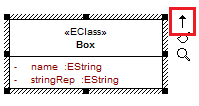
\includegraphics[width=0.4\textwidth]{ea_quickLink}
	\caption{Quick Link is a central gesture in EA}
	\label{ea:quicklink}
\end{figure}
\FloatBarrier

\item[$\blacktriangleright$] Click this black arrow and `pull' to the element you wish to link to. To start, quick-link from \texttt{Box} to \texttt{Partition}.
In the context menu that appears, select ``Create Bidirectional EReference'' (Fig.~\ref{ea:ereference}).

\begin{figure}[htbp]
	\centering
  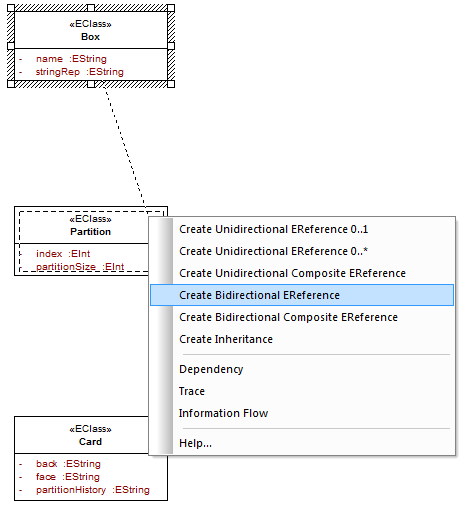
\includegraphics[width=0.6\textwidth]{ea_eReferenceBidirectional}
	\caption{Create an EReference via Quick Link}
	\label{ea:ereference}
\end{figure}
\FloatBarrier

\item[$\blacktriangleright$] Double click the EReference to invoke a dialogue. In this window you can adjust all relevant settings. Feel free to leave the
\texttt{Name} value blank - this property is only used for documentation purposes, and is not relevant for code generation.

\item[$\blacktriangleright$] Within this dialogue, go to ``Source Role,'' and compare the relevant values in Fig.~\ref{ea:role_source} for the \emph{source}
end of the EReference (the \texttt{Box} role). As you can see, the default source is set to the EClass you linked from, while the default target
is the EClass you linked to. In this window, do not forget to confirm and modify the \texttt{Role}, \texttt{Navigability}, \texttt{Multiplicity}, and
\texttt{Aggregation} settings for the source as required. Repeat the process for the \texttt{Target Role} (Fig.~\ref{ea:role_target}).

\vspace{0.5cm}

\begin{figure}[htbp]
	\centering
    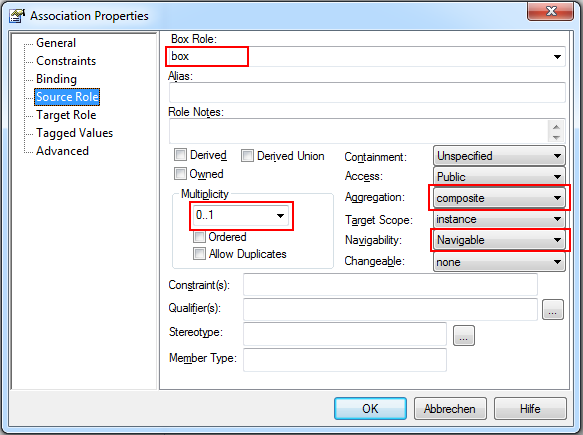
\includegraphics[width=0.9\textwidth]{ea_assocPropsSource}
	\caption{Properties for the source role of an EReference}
	\label{ea:role_source}
\end{figure}

\begin{figure}[htbp]
	\centering
	  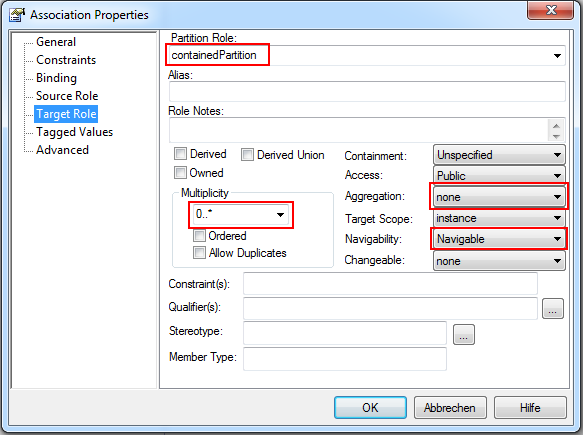
\includegraphics[width=0.9\textwidth]{ea_assocPropsTarget}
	\caption{Properties for the target role of an EReference}
	\label{ea:role_target}
\end{figure}

\end{itemize}

To review these properties, the first value you edited was the role name. The \texttt{Navigation} value should have been automatically set to
\texttt{Na\-vi\-ga\-ble}. Without these two settings, getter and setter methods will not be generated.

Next, you set the \texttt{Multiplicity} value.  In your source role (\texttt{Box}), you have allowed the creation of up to one target (\texttt{Partition})
reference for every connected source (\texttt{box}). This means you could not have a single target connected to two sources (i.e., one partition that belongs to
two boxes). In the target (\texttt{Partition}) role, you have specified that any source (in our case, \texttt{box}) can have any positive-sized number of targets.
Figure~\ref{fig:sketch_roles} sketches this schematically.

\vspace{0.5cm}

\begin{figure}[htbp]
	\centering
    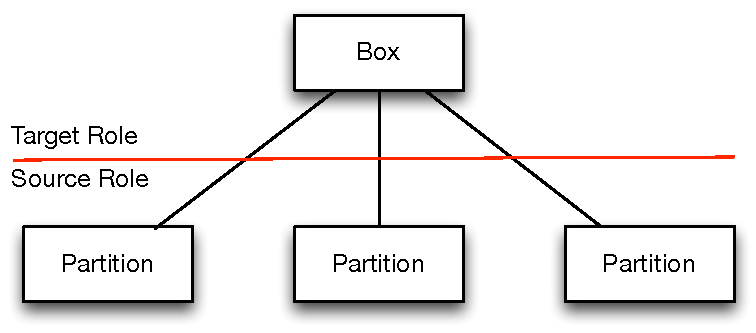
\includegraphics[width=0.6\textwidth]{sketch_multiplicities.pdf}
	\caption{The target and source roles of Leitner's Learning Box}
	\label{fig:sketch_roles}
\end{figure}
\FloatBarrier

Finally, you set the \texttt{Aggregation} value. In this case, \texttt{box} is a container for \texttt{Partition}s, and \texttt{containedPartition} is
consequently not.

\begin{itemize}
\item[$\blacktriangleright$] Take a moment to review how the \texttt{Aggregration} settings extend the \texttt{Multiplicity} rules. If you've done everything
right, your metamodel should now resemble Figure~\ref{ea:ereference_completed}, with a single \emph{bidirectional EReference} between \texttt{Box} and
\texttt{Partition}.

\vspace{1cm}

\begin{figure}[htbp]
	\centering
  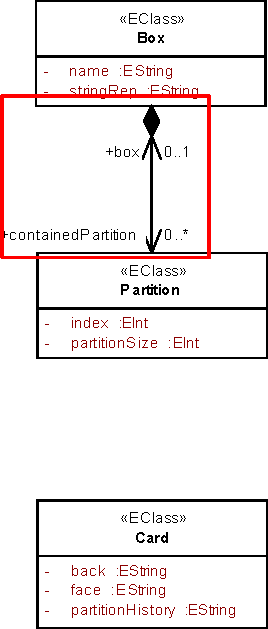
\includegraphics[width=0.35\textwidth]{ea_relationBoxPartition.pdf}
	\caption{\texttt{Box} contains \texttt{Partition}s}
	\label{ea:ereference_completed}
\end{figure}
\FloatBarrier

\item[$\blacktriangleright$] Following the same process, create two unidirectional self-EReferences for \texttt{Partition} (for next and previous \texttt{Partitions}), and a second bidirectional composite
EReference\footnote{To be precise, \emph{all} EReferences in Ecore are actually unidirectional. A ``bidirectional'' EReference in our metamodel is really two
mapped EReferences that are opposites of each other. We however, believe it is simpler to handle these pairs as single EReferences, and prefer this
concise concrete syntax.} between \texttt{Partition} and \texttt{Card} (Fig.~\ref{ea:ereferences_all}). 

\vspace{1cm}

\begin{figure}[htbp]
	\centering
  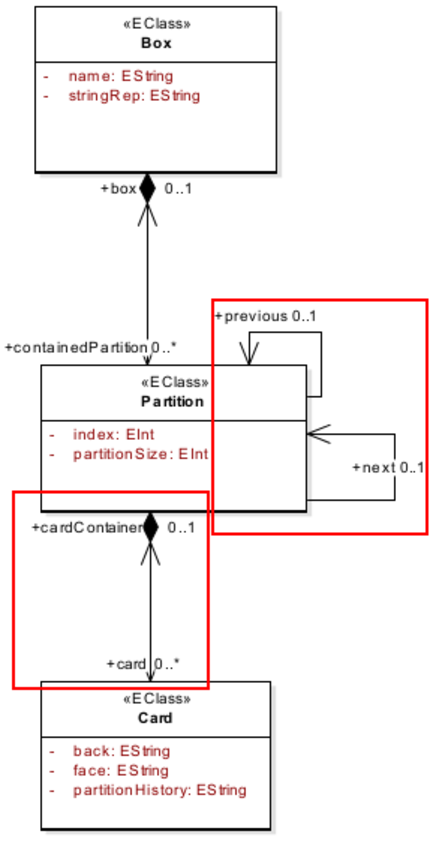
\includegraphics[width=0.7\textwidth]{ea_classAttributes}
	\caption{All relations in our metamodel}
	\label{ea:ereferences_all}
\end{figure}
\FloatBarrier

\vspace{1cm}

\item[$\blacktriangleright$] You'll notice that the connection between \texttt{Card} and \texttt{Partition} is similar to that between \texttt{Partition} and
\texttt{Box}. This makes sense as a partition should be able to hold an unlimited amount of cards, but a card can only belong to one partition at a time.

\vspace{1cm}

\item[$\blacktriangleright$] Export your diagram to Eclipse and refresh your workspace. Your Ecore metamodel file in ``model/LearningBoxLanguage.ecore" should now resemble Figure~\ref{eclipse:model_allClasses}.

\vspace{1cm}

\begin{figure}[htbp]
	\centering
  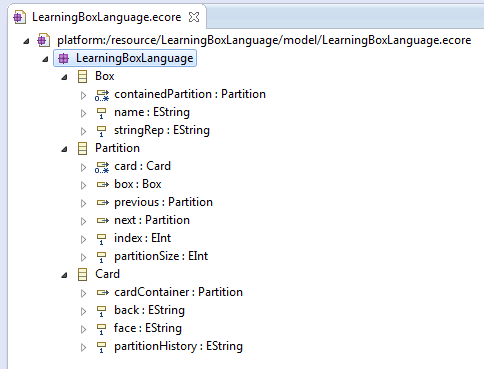
\includegraphics[width=0.7\textwidth]{eclipse_modelDeclaredClasses}
	\caption{Refreshed Ecore file with all EReferences}
	\label{eclipse:model_allClasses}
\end{figure}

\vspace{1cm}

\item[$\blacktriangleright$] All the required attributes and references for your learning box have now been set up. We encourage you to see how these are
declared in the textual syntax, starting on the immediate next page. In particular, check out Fig.~\ref{eclipse:allReferences}, where each EClass is fully
declared, and Fig.~\ref{eclipse:bothConstraints}, where bidirectionality is explicitly specified as a constraint.

\jumpSingle{static:methods vis}

\end{itemize}
